\subsection{Passive and Active Inductor CTLE}
\label{sec:inductor_ctle}

Passive shunt-peaking CTLEs enhance the frequency response by incorporating inductors in the load network to introduce additional zeros and complex poles. This approach extends the bandwidth and increases peaking gain compared to conventional SD-CTLEs. However, the use of passive inductors presents significant implementation challenges in integrated circuit design.

\newpage
\subsubsection{Passive Shunt-Peaking CTLE}
\label{subsec:passive_shunt_peaking}

The passive shunt-peaking CTLE extends the conventional SD-CTLE architecture by adding a pair of passive inductors $L_P$ in series with the load resistors $R_L$, as shown in Figure~\ref{fig:passive_shunt_peaking_schematic}.

\begin{figure}[H]
    \centering
    \begin{subfigure}[b]{0.45\textwidth}
        \centering
        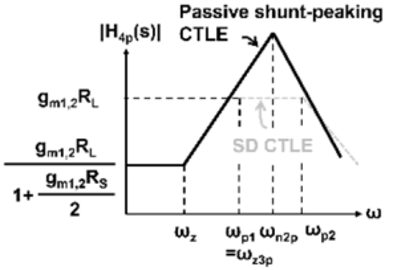
\includegraphics[width=\textwidth]{img/CTLE_img/passive_ind_assymptotic.png}
        \caption{Asymptotic response comparison}
        \label{fig:passive_assymptotic}
    \end{subfigure}
    \hfill 
    \begin{subfigure}[b]{0.45\textwidth}
        \centering
        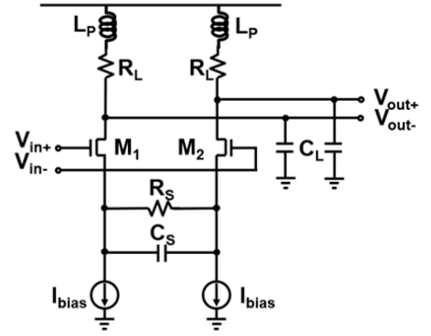
\includegraphics[width=\textwidth]{img/CTLE_img/passive_ind schematic.png}
        \caption{Passive shunt-peaking schematic}
        \label{fig:passive_shunt_peaking_schematic}
    \end{subfigure}
    \caption{Comparison of passive shunt-peaking response and architecture.}
    \label{fig:passive_comparison_full}
\end{figure}

The transfer function for the passive shunt-peaking CTLE introduces an additional zero $\omega_{3p}$ and a pair of complex-conjugate poles:

\[
H_{4p}(s) = \left( -\frac{g_{m1,2}R_L}{1 + \frac{g_{m1,2}R_s}{2}} \right) \cdot \frac{1 + \frac{s}{\omega_{z}}}{1 + \frac{s}{\omega_{p}}} \cdot \frac{1 + \frac{s}{\omega_{3p}}}{1 + \frac{2\zeta_{2p}}{\omega_{3p}} s + \frac{s^2}{\omega_{2p}^2}}
\]

where:
\[
\omega_{3p} = \frac{R_L}{L_P}, \quad \omega_{n2p} = \frac{1}{\sqrt{L_P C_L}}, \quad \zeta_{2p} = \frac{R_L}{2} \sqrt{\frac{C_L}{L_P}}
\]

As shown in Figure~\ref{fig:passive_assymptotic}, the additional zero $\omega_{3p}$ can cancel the dominant pole $\omega_{p1}$, while the complex poles at $\omega_{n2p}$ create a resonant peak that enhances high-frequency gain.

\newpage
\subsubsection*{Limitations and Practical Considerations}

Despite its performance advantages, passive shunt-peaking CTLEs face critical limitations:

\begin{itemize}
    \item \textbf{Area Consumption}: Passive inductors consume significant silicon area, increasing chip cost.
    \item \textbf{Limited Tunability}: Minimal post-fabrication tuning capability compared to active components.
\end{itemize}

\subsubsection{Active Inductor CTLE}
\label{subsec:active_ind_ctle}

Active inductor CTLEs provide an area-efficient alternative to passive shunt-peaking implementations by replacing bulky passive inductors with transistor-based active circuits that emulate inductive behavior. As noted in the literature, "an inductive-peaking CTLE involves a pair of active inductors enhances area efficiency" while maintaining comparable performance benefits.

\subsubsection*{Circuit Architecture and Operation}

\begin{figure}[H]
    \centering
    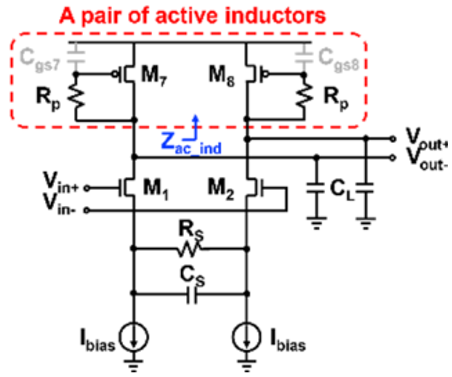
\includegraphics[width=0.6\textwidth]{img/CTLE_img/active_schematic.png}
    \caption{Active inductor CTLE architecture implementing inductive peaking with transistor-based active inductors [H. Hsu TCAS I '25].}
    \label{fig:active_ind_schematic}
\end{figure}

The active inductor CTLE, shown in Figure~\ref{fig:active_ind_schematic}, replaces passive inductors with active inductor cells formed by transistors M7, M8 and feedback resistors $R_P$. 
\newpage
The impedance looking into the active inductor is given by:

\[
Z_{ac\_ind} \approx \frac{1}{g_{m7,8}} + s \cdot \frac{C_{gs7,8}}{g_{m7,8}^2}
\]

where the effective inductance is $L_{\text{eff}} = \frac{C_{gs7,8}}{g_{m7,8}^2}$. The feedback resistor $R_P$ increases high-frequency impedance and effectively acts as an impedance peaking element, enhancing the overall gain at the target frequencies.

\subsubsection*{Frequency Response Analysis}

The transfer function for the active inductor CTLE incorporates the effects of the active inductive load:

\[
H_4(s) = \left( \frac{\frac{g_{m1,2}}{g_{m7,8}}}{1 + \frac{g_{m1,2}R_s}{2}} \cdot \frac{1 + \frac{s}{\omega_z}}{1 + \frac{s}{\omega_{p1}}} \right) \cdot \left( \frac{1 + \frac{s}{\omega_{z3}}}{1 + \frac{2\zeta_2}{\omega_{n2}} s + \frac{s^2}{\omega_{n2}^2}} \right)
\]

where the key frequency parameters are:

\[
\begin{aligned}
\omega_{n2} &= \sqrt{\frac{g_{m7,8}}{R_P C_{gs7,8} C_L}}, &\quad
\zeta_2 &= \frac{\omega_{n2}(C_L + C_{gs7,8})}{2g_{m7,8}}, &\quad
\omega_{z3} &= \frac{1}{R_P C_{gs7,8}}
\end{aligned}
\]

\begin{figure}[H]
    \centering
    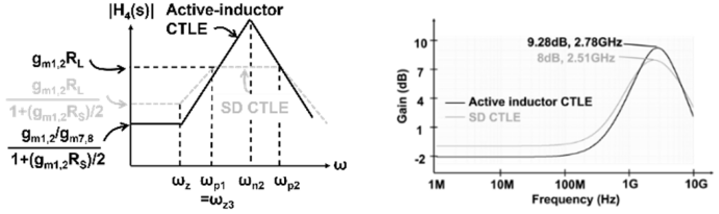
\includegraphics[width=\textwidth]{img/CTLE_img/active_assymptotic_and_real.png}
    \caption{Frequency response comparison showing active inductor CTLE compared to SD-CTLE [H. Hsu TCAS I '25].}
    \label{fig:active_ind_response}
\end{figure}

As shown in Figure~\ref{fig:active_ind_response}, the active inductor CTLE achieves 9.28 dB peaking at 2.78 GHz, representing a 16\% improvement in peaking gain and 10.8\% increase in peaking frequency compared to conventional SD-CTLE. The asymptotic plot illustrates how the additional zero $\omega_{z3}$ and complex poles at $\omega_{n2}$ create enhanced high-frequency response.

\subsubsection*{Design Knobs and Tunability}

The active inductor CTLE offers enhanced tunability through several key parameters:

\begin{itemize}
    \item \textbf{Transistor Widths ($W_{7,8}$)}: Control the transconductance $g_{m7,8}$, which directly determines the effective inductance $L_{\text{eff}} = \frac{C_{gs7,8}}{g_{m7,8}^2}$ and the natural frequency $\omega_{n2}$.
     
    \item \textbf{Feedback Resistance ($R_P$)}: Increasing $R_P$ enhances the peak gain by boosting high-frequency impedance. This parameter affects both $\omega_{n2}$ and $\omega_{z3}$.
     
    \item \textbf{Active Inductor Bias}: Controls the operating point of M7 and M8, allowing dynamic adjustment of the inductive characteristics.
\end{itemize}

\subsubsection*{PVT Variations and Design Margins}

\begin{figure}[H]
    \centering
    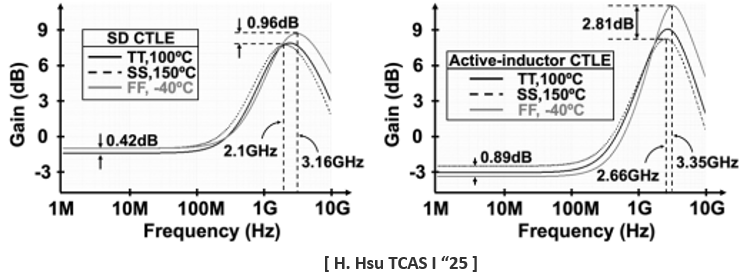
\includegraphics[width=\textwidth]{img/CTLE_img/active pvt.png}
    \caption{PVT variations affecting SD-CTLE and active inductor CTLE responses across process corners.}
    \label{fig:active_ind_pvt}
\end{figure}

As shown in Figure~\ref{fig:active_ind_pvt}, the impedance formed by the pair of active inductors encounters significant PVT shifts:

\begin{itemize}
    \item \textbf{Fast-Fast (FF) Corner at -40°C}: Higher $g_m$ increases peaking gain to 9.28 dB at 2.86 GHz but reduces stability margin.
    \item \textbf{Slow-Slow (SS) Corner at 150°C}: Reduced $g_m$ decreases peaking to 8.89 dB at 3.35 GHz, potentially under-equalizing the channel.
    \item \textbf{Typical-Typical (TT) Corner at 100°C}: Represents the nominal design condition with balanced performance.
\end{itemize}

The active inductor CTLE shows reduced PVT sensitivity compared to SD-CTLE, with peaking gain variation of 0.39 dB (4.2\%) versus 0.96 dB (12\%) for SD-CTLE across corners. However, certain design margin is still required to account for these variations.

\subsubsection*{Design Trade-offs}

\begin{table}[H]
\centering
\caption{Active Inductor CTLE Design Trade-offs}
\label{tab:active_ind_tradeoffs}
\begin{tabular}{ >{\raggedright\arraybackslash}p{0.13\textwidth} 
                 >{\raggedright\arraybackslash}p{0.28\textwidth} 
                 >{\raggedright\arraybackslash}p{0.25\textwidth} 
                 >{\raggedright\arraybackslash}p{0.35\textwidth} }
\toprule
\textbf{Parameter} & \textbf{Benefit} & \textbf{Risk} & \textbf{Design Guideline} \\
\midrule
$W_{7,8}$ & Controls $L_{\text{eff}}$ and peaking & PVT sensitivity, area & Size for nominal $g_m$ with 20\% margin \\
\midrule
$R_P$ & Increases peak gain, sets $\omega_{z3}$ & Stability risk, noise & Optimize for target peaking frequency \\
\midrule
Active Inductor & Area efficiency, tunability & Complexity, power & Verify $\zeta_2 > 0.7$ for stability \\
\midrule
$g_{m7,8}$ & Determines $\omega_{n2}$ and $\zeta_2$ & PVT variations & Implement bias compensation \\
\bottomrule
\end{tabular}
\end{table}